\documentclass[12pt]{article}

% 1. Carregar os pacotes de idioma e fontes PRIMEIRO
\usepackage[T1]{fontenc}
\usepackage[utf8]{inputenc}
\usepackage[brazilian]{babel}

% 2. Carregar o template da SBC DEPOIS
\usepackage{sbc-template}

% 3. Demais pacotes
\usepackage{graphicx,url}
\usepackage[numbers]{natbib}
\usepackage{tabularx}
\usepackage{hyperref}
\usepackage{xspace}

\newcommand{\offscan}{\textit{OffScan}\xspace}
\newcommand{\mitreattack}{MITRE ATT\&CK\xspace}
     
\sloppy

\title{OffScan: Uma Ferramenta para Testes Ofensivos em Redes Wi-Fi}

\author{
Oliver Ribeiro Calazans Jeronimo,
Teobaldo Adelino Dantas de Medeiros
}

\address{
Instituto Federal do Rio Grande do Norte (IFRN), Campus Natal Central\\ Avenida Senador Salgado Filho, nº 1559 -- 59015-000 -- Natal -- RN -- Brazil
\email{
  oliver.calazans@academico.ifrn.edu.br, teobaldo.dantas@ifrn.edu.br
}
}

\makeatletter
\let\bbl@normalsf\relax
\let\normalsfcodes\relax
\makeatother

\begin{document}
\maketitle


\begin{abstract}
This paper presents \offscan, a tool for offensive Wi-Fi network testing implemented in Go. Developed with a focus on modularity, performance, and autonomy, the tool integrates functionalities such as multi-layer host discovery, packet capture and injection, and cryptographic attack. OffScan represents a practical contribution to the offensive security ecosystem, offering a foundation for future developments.
\end{abstract}



\begin{abstract}
Este artigo apresenta o \offscan, uma ferramenta para testes ofensivos de redes Wi-Fi implementada em Go. Desenvolvida com foco em modularidade, desempenho e autonomia, a ferramenta integra funcionalidades como descoberta de hosts em diferentes camadas, captura e injeção de pacotes, e ataques a criptografia. O OffScan representa uma contribuição prática ao ecossistema de segurança ofensiva, oferecendo uma base para desenvolvimentos futuros.
\end{abstract}
\section{Introdução}
Com o crescimento exponencial da conectividade e da complexidade das infraestruturas de rede, a segurança cibernética tornou-se uma preocupação crítica para organizações e indivíduos. Os ataques evoluíram em sofisticação, utilizando técnicas mapeadas pelo \mitreattack e explorando vulnerabilidades criticamente ativas no mercado, como as catalogadas pelo CISA KEV, exigindo ferramentas eficazes de teste de penetração e análise de vulnerabilidades que permitam avaliar proativamente a resiliência dos sistemas.

Neste contexto, este projeto apresenta o desenvolvimento da ferramenta \offscan, uma solução ofensiva para redes Wi-Fi escrita em Go.

O \offscan foi desenvolvido com foco em modularidade, desempenho e autonomia, reduzindo as dependências externas por meio do uso da linguagem Go, que possui bibliotecas robustas para redes de computadores. A ferramenta incorpora funcionalidades para testes ofensivos, incluindo descoberta de dispositivos e redes, captura e injeção de pacotes, e técnicas específicas para redes sem fio, como ataques a protocolos e criptografia.

Este relatório documenta o processo de desenvolvimento do \offscan, detalhando a evolução da arquitetura, as funcionalidades implementadas e os resultados obtidos em ambiente controlado. Além disso, discute as lições aprendidas, as limitações identificadas e as direções futuras para o projeto.
\section{Fundamentação teórica}

A segurança ofensiva de redes Wi-Fi compreende um conjunto de técnicas e metodologias destinadas a identificar, explorar e relatar vulnerabilidades em sistemas e infraestruturas de rede, com o propósito proativo de fortalecer suas defesas. Diferente da segurança defensiva, que visa proteger sistemas contra ataques, a abordagem ofensiva simula as ações de adversários reais para avaliar a resiliência dos mecanismos de proteção. A área da segurança ofensiva vem ganhando atenção por se mostrar eficiente e ajudar no treinamento de equipes e refinamento nas técnicas de detecção e prevenção de ataques.

Neste projeto, a segurança ofensiva é aplicada por meio de uma ferramenta que realiza varreduras, enumeração e ataques em ambientes sem fio. Técnicas como flooding (inundação) de beacons, deautenticação de dispositivos pelo protocolo IEEE 802.11, spoofing (falsificação) de endereços IP/MAC são fundamentais para o teste de penetração, explorando falhas em protocolos, configurações inadequadas ou limitações de implementação.

Para a implementação de uma ferramenta ofensiva eficaz, é essencial o domínio dos protocolos de rede que atuam em diversas camadas do modelo TCP/IP, em especial na camada 2, onde há a presença do protocolo IEEE 802.11. O ICMP (\textit{Internet Control Message Protocol}), utilizado para diagnóstico, serve de base para enumeração e busca de informações de dispositivos. O padrão IEEE 802.11 (Wi-Fi) é essencial, sendo explorado por meio da captura de beacons e ataques de desautenticação, que manipulam quadros de gerenciamento.
\section{Metodologia}
Esta seção descreve a metodologia adotada para o desenvolvimento da ferramenta \offscan, detalhando o ambiente de desenvolvimento, a arquitetura do sistema, as funcionalidades implementadas, os procedimentos de teste e os métodos de coleta de dados.

\subsection{Ambiente de Desenvolvimento}
O desenvolvimento do \offscan foi realizado em ambiente Linux (distribuições Debian 12). Este sistema operacional foi selecionado devido ao suporte nativo a \textit{sockets} brutos (\textit{raw sockets}) e chamadas de sistema (\textit{syscalls}) de baixo nível, requisitos mandatórios para operações ofensivas de rede. 

A linguagem de programação Go foi selecionada para o desenvolvimento desta ferramenta devido a características técnicas que se alinham aos requisitos de sistemas de segurança ofensiva. A simplicidade de sua sintaxe reduz a complexidade do código, facilitando a manutenção e a depuração do software. Por ser uma linguagem compilada diretamente para código de máquina, Go apresenta desempenho em tempo de execução adequado para operações de alta velocidade, como varreduras de diversas redes simultaneamente. Adicionalmente, o modelo de concorrência baseado em Goroutines viabiliza a execução eficiente de tarefas paralelas, enquanto seu ecossistema nativo oferece suporte à manipulação de protocolos de redes de computadores. Desse modo, os recursos da linguagem suprem as demandas de desempenho, concorrência e portabilidade necessárias para a arquitetura do \offscan.

As principais ferramentas e bibliotecas utilizadas incluem:
\begin{itemize}
    \item \textbf{Adaptador de Rede Sem Fio}: Dispositivo de hardware equipado com \textit{chipset} homologado para suporte nativo ao modo monitor (\textit{monitor mode}) e injeção de pacotes (\textit{packet injection}), condições indispensáveis para a interceptação de quadros de gerenciamento e execução de ataques na camada de enlace.

    \item \textbf{Sistema Operacional Linux}: Ambiente de execução obrigatório para o funcionamento da ferramenta, uma vez que a implementação depende de chamadas de sistema (\textit{syscalls}) específicas do kernel Linux para captura de pacotes, manipulação de \textit{sockets} e alteração das configurações da interface de rede sem fio (como a ativação do modo monitor).
    
    \item \textbf{Compilador Go}: Sistema de compilação e gerenciador de pacotes do ecossistema Go, utilizando a versão 1.25.0 ou superior.
    
    \item \textbf{golang.org/x/sys}: Repositório oficial do ecossistema Go (externo à biblioteca padrão), empregado para realizar chamadas de sistema diretas e configurar os \textit{sockets}.
\end{itemize}

\subsection{Arquitetura da Ferramenta}
A arquitetura do \offscan segue um padrão de projeto modular, organizado em componentes especializados que colaboram de forma coordenada para executar operações ofensivas. Seus principais módulos consistem em:

\begin{itemize}
    \item \textbf{Motores (\textit{Engines})}: Blocos lógicos que coordenam e executam as operações fim da ferramenta, utilizando as funções dos demais módulos para consolidar rotinas de varredura ou ataque.
    
    \item \textbf{Construtores de Pacotes/Quadros}: Componentes responsáveis pela montagem manual de pacotes de rede em múltiplas camadas (ARP, IP, TCP, ICMP) e de quadros do padrão IEEE 802.11.
    
    \item \textbf{Sockets Brutos}: Módulo encarregado do envio direto dos pacotes e quadros injetados na interface de rede.
    
    \item \textbf{Sniffer}: Componente encarregado da captura e interceptação de pacotes ou quadros em tempo real diretamente de uma interface de rede.
    
    \item \textbf{Dissecadores de Pacotes/Quadros}: Funções responsáveis pela decodificação e extração de campos e metadados dos pacotes e quadros capturados.
    
    \item \textbf{Geradores}: Blocos lógicos encarregados de produzir iteradores e valores pseudoaleatórios (como portas de origem ou identificadores).
    
    \item \textbf{Provedor de Informações}: Subsistema encarregado de coletar metadados das interfaces físicas de rede e parâmetros operacionais do sistema subjacente.
    
    \item \textbf{Modelos (\textit{Models})}: Componente que centraliza a definição de estruturas (\textit{structs}) e tipos customizados do sistema, atuando na padronização de dados, facilitação da legibilidade e garantia de consistência durante o desenvolvimento.
    
    \item \textbf{Utilitários}: Funções auxiliares isoladas que fornecem rotinas genéricas e reutilizáveis em múltiplos módulos do sistema.
\end{itemize}

\subsection{Fluxo de Execução}
A ferramenta opera como uma aplicação de interface de linha de comando (CLI), na qual cada funcionalidade é invocada por meio de subcomandos específicos. O fluxo geral compreende quatro etapas sequenciais: (1) análise sintática (\textit{parsing}) dos argumentos e parâmetros de entrada; (2) inicialização e acoplamento dos módulos exigidos; (3) execução do motor principal correspondente à operação requisitada (varredura, ataque ou análise); e (4) exibição estruturada dos resultados ao usuário.

\section{Funcionalidades}

A ferramenta tem seu foco em ataques a redes Wi-Fi. Mas, também conta com alguns scanners que são úteis para fornecer informações para serem usadas nos ataques. Elas são:


\subsection{\textbf{Ataque de Desautenticação}}
Esse ataque explora uma vulnerabilidade fundamental no protocolo 802.11, que gerencia as comunicações Wi-Fi. Ele é possível devido a duas características principais do protocolo:

\begin{itemize}
    \item Os quadros de gerenciamento, como os de autenticação e desautenticação, são enviados sem criptografia, exceto nas redes com WPA3 e WPA2 que usam o padrão 802.11w.

    \item O padrão Wi-Fi original não exige que os dispositivos verifiquem se um quadro de desautenticação foi enviado pelo ponto de acesso legítimo.
\end{itemize}

Um atacante pode enviar quadros de desautenticação forjados para um dispositivo (cliente) e/ou para o ponto de acesso (AP), fingindo ser a outra parte legítima da conexão. O dispositivo e/ou o AP aceita esses quadros falsificados como se fossem legítimos, pois não há um mecanismo de verificação de origem. Essa falha é usada em combinação com outros ataques como o ataque \texttt{kr00k} \cite{kr00k}, \texttt{KRACK} \cite{krack} e \texttt{evil-twin} \cite{evil-twin}.

O \offscan usa dessas falhas para executar o ataque. Ele cria os frames de desautenticação usando as informações passadas pela linha de comando e envia os frames em um loop infinito para o host alvo, se passando pelo AP, e para o AP, se passando pelo host alvo.

Essa falha foi descoberta em 2002 mas documentada em 2003. Sua primeira aparição foi no artigo \citet{80211-flaws} ainda em 2003. Mas essa falha ainda se mostra relevante pois são portados CVEs relacionados a ela, como o CVE-2026-26048 \cite{deauth-protecless}




\subsection{\textbf{Flooder de Beacons}}
Beacons são quadros (frames) enviados por roteadores de redes Wi-Fi para se apresentarem e enviarem informações necessárias para que dispositivos possam se conectar as suas redes sem fio.

O inundador de beacons cria vários desses beacons com informações falsas para que os dispositivos ao alcance recebem esses beacons e os processem como se fossem redes reais. Isso faz com que a lista de redes disponíveis fique maior e confunda os usuários, o que se enquadra em um ataque de confusão de SSID \cite{confusion-attack}. Uma das informações que o inundador usa é nome de rede (BSSID) que pode ser de uma rede real ou não. Para evitar filtragem de redes pela repetição do mesmo BSSID, o código cria variações do nome passado, alterando algumas letras de maiúscula para minúscula, e o inverso também. Assim como o ataque de desautenticação, esse flooder é comumente usado em conjunto com outras técnicas.

Esse flooder pode ser usado para ataques DoS em dispositivos IoT devido as limitações de hardware e/ou falhas no software. Esses ataques podem ocorrer por diferentes motivos como por consumo descontrolado de recursos \cite{cwe400}, alocação de recursos sem limites \cite{cwe770} e estouro de buffer baseado em pilha \cite{cwe121}.



\subsection{\textbf{Descoberta de dispositivos}}
Apesa de não ser um ataque, e sim uma técnica de reconhecimento \cite{ip-scanning}, ele é extremamente útil para serem usadados em ataque e/ou tomadas de decisão. Essa funcionalidade usa uma técnica de enviar pacotes especificos e analisar as respostas recebidas. No caso de uma escaneamento ativo.

A descoberta de dispositivos do \offscan envia pacotes ARP (para endereços locais), ICMP e TCP (por padrão, é possível escolher um ou todos os três serão usados para todos os IPs da rede, ou de um range especificado. O gerador recebe o CIDR (baseado na interface que será usada) ou um range específico e calcula todos os IPs possíveis e entrega um iterador para ser usado nos probes.

Durante o envio dos pacotes, um sniffer fica capturando as respostas em uma \textit{goroutine} (\textit{thread}) separada. Ele possui um filtro BPF (\textit{Berkley Packet Filter}) que busca por pacotes IPv4 e que contenham endereços de IP dentro do range especificado por um CIDR. Esse CIDR é criado basedo no primeiro e último IPs gerados pelo módulo \texttt{Ipv4Iter}. Assim, deixando a captura por pacotes mais especifica.



\subsection{\textbf{Descoberta de dispositivos na camada 2 (IEEE 802.11)}}

Essa técnica de descoberta de dispositivos tem objetivo semelhante ao da abordagem baseada em pacotes TCP/IP, porém difere na forma de operação, no alcance e no tipo de informação obtida.

Com a interface de rede em modo monitor, um sniffer captura dois tipos de quadros IEEE 802.11: \textit{beacons} e \textit{data frames}. A partir desses quadros, é possível descobrir quais dispositivos estão ativos no entorno e a quais redes eles estão conectados.

Os \textit{beacons} são enviados pelos pontos de acesso (APs) para anunciar suas redes. Deles, extraem-se apenas o SSID, o BSSID e o canal. Já os \textit{data frames} são trocados entre dispositivos e APs após o estabelecimento de uma conexão. Desses quadros, obtêm-se o endereço MAC do dispositivo e o BSSID.

Ao cruzar o BSSID presente nos \textit{data frames} com o BSSID dos \textit{beacons}, é possível identificar a qual rede cada AP pertence e quais dispositivos estão associados a ele.

Essa abordagem de descoberta é passiva e extremamente silenciosa. Ela só é viável porque os cabeçalhos dos quadros IEEE 802.11 não são criptografados — eles precisam ser legíveis para que os dispositivos possam verificar se cada quadro é destinado a eles ou deve ser descartado. Além disso, evitar a decriptação reduz o tempo de processamento e aumenta a vazão da rede.



\subsection{\textbf{Mapeador de redes Wi-Fi}}
O reconhecimento das redes Wi-Fi está cada vez mais sendo usado por atacantes por ser um vetor/porta inicial de ataque \cite{wifi-vec}. Buscar informações sobre as redes disponíveis pode revelar informações úteis para outras .

O mapedor de redes Wi-Fi tem como objetivo mostrar informações de cada rede wifi ao alcance. Essas informações são úteis para o ataque como o de desautenicação e outros.

As informações capturadas são:
\begin{itemize}
    \item BSSID (Endereço MAC)
    \item SSID (Nome da rede)
    \item Canal
    \item Frequência
    \item Padrão técnico (802.11X)
    \item Criptografia
\end{itemize}

Ele inicia o sniffer na interface e entra em um loop que fica alterando o canal da interface periodicamente. Após escanar cada interface, o sniffer é fechado e os pacotes são processados e as informações são formatadas e apresentadas.



\subsection{\textbf{Informações de Rede e Interface}}
Essa funcionalidade tem como objetivo mostrar algumas informações da interface e da rede, se estiver conectada, sem a necessidade de escanar a rede. As informações que são apresentadas são:

\begin{itemize}
    \item Nome da interface
    \item Estado da interface (UP, DOWN, ETC)
    \item Tipo (Ethernet, Wireless, etc)
    \item Endereço MAC
    \item Endereço de IP
    \item Endereço da rede e mascara (CIDR)
    \item Quantidade de IPs válidos
    \item MTU (Unidade Máxima de Transmissão)
    \item Endereço MAC do gateway
    \item Endereço de IP do gateway
\end{itemize}

Essas informações são buscadas de origens diferentes. Nome, estado, tipo, MAC e MTU são copiadas dos arquivos \texttt{/sys/class/net/<interface>}. Já os endereços de IP e MAC do gateway são copiados de arquivos que ficam nos diretórios \texttt{/proc/net/}. Já o IP e o endereço da rede com a máscara são conseguidos atravez de chamadas ao sistema usando a crate \texttt{libc}. E a quantidade de IPs válidos é calculada através do CIDR.

Essas informações são úteis para serem usadas pelos outros comandos e/ou para tomada de decisão.
\section{Resultados}
Os resultados da execução de cada função mostra como o está o funcionamento do sua funcionalidades. 



\subsection{Amostra das execuções}



\subsubsection{Ataque de desautenticação}
O ataque demonstrou ser eficaz em provocar a desassociação do cliente do ponto de acesso. O tempo de reação do dispositivo alvo fica entre 10 e 30 segundos.
\begin{figure}[h]
    \centering
    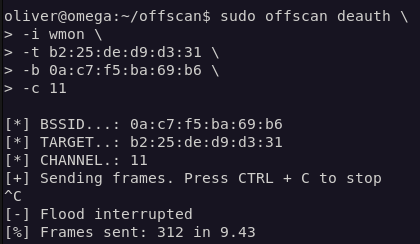
\includegraphics[width=0.45\textwidth]{fotos/deauth.png}
    \caption{Execução do mapeador de rede}
\end{figure}



\subsubsection{Descoberta de dispositivos}
No exemplo abaixo, apenas o comando para descobrir dispositivos na rede foi informado. Com isso, a interface padrão é usada e a partir do IP e da mascara da rede, todos os IPs da rede são calculados para serem escaneados.
\begin{figure}[h]
    \centering
    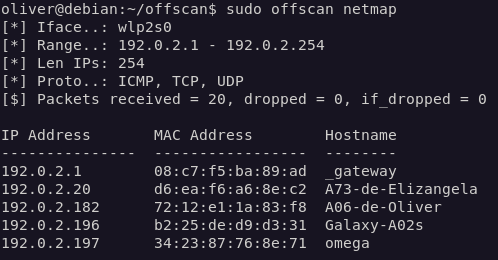
\includegraphics[width=0.46\textwidth]{fotos/hostdisc.png}
    \caption{Execução do mapeador de rede}
\end{figure}



\subsubsection{Informações de Rede e Interface}
No exemplo abaixo o comando \texttt{info} foi executado. Ele mostra informações da interface que foi escolhida e da rede ao qual está conectada, se estiver.
\begin{figure}[h]
    \centering
    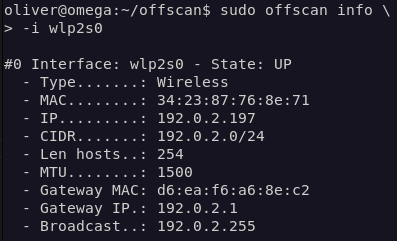
\includegraphics[width=0.46\textwidth]{fotos/info.png}
    \caption{Execução do comando \texttt{info}}
\end{figure}



\subsubsection{Mapeador de redes Wi-Fi}
No exemplo desse comando foram alterados o nome da rede (SSID) e parte do BSSID de cada rede para preservar a privacidade. A imagem abaixo mostra como o comando mostra as informações que pegou de cada rede Wi-Fi.
\begin{figure}[h]
    \centering
    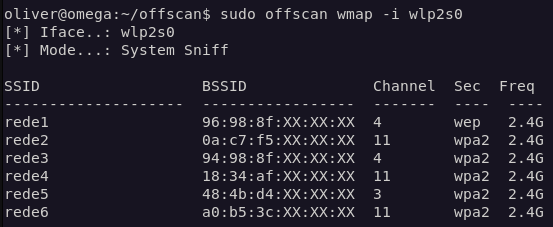
\includegraphics[width=0.46\textwidth]{fotos/wmap.png}
    \caption{Execução do mapeador de redes Wi-Fi}
\end{figure}



\subsubsection{Flooder de beacons}
O flooder de beacons se mostrou muito eficiente como mostra a imagem abaixo. Nela, é possível ver algumas das muitas redes inexistentes que os beacons transmitiram.
\begin{figure}[h]
    \centering
    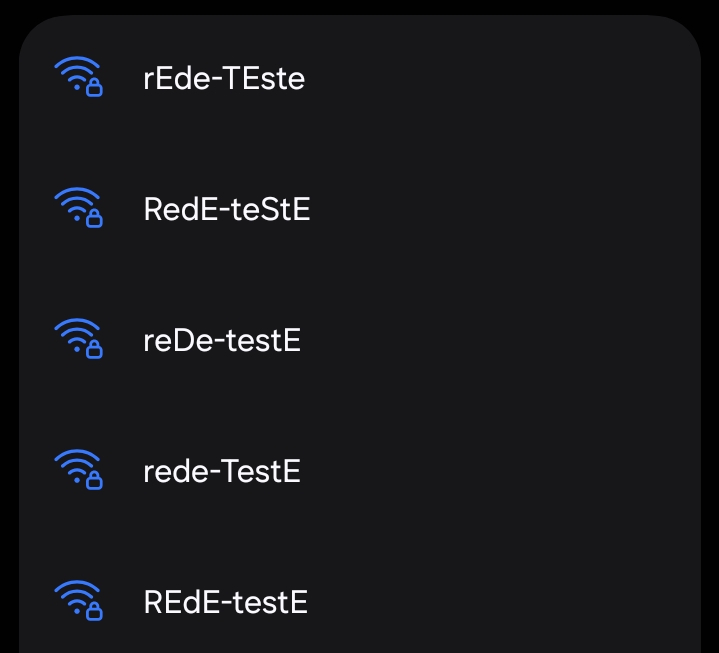
\includegraphics[width=0.46\textwidth]{fotos/beacon.jpg}
    \caption{Execução do flooder de beacons}
\end{figure}



\subsection{Análise dos resultados}
Com base nas execuções, observou-se que: 

\begin{itemize}
    \item \textbf{Flooder de beacons}: A taxa de envio foi limitada intencionalmente para evitar a saturação do espectro e permitir a visualização clara das redes falsas. Apesar dessa limitação, a funcionalidade mostrou-se eficaz, com múltiplos dispositivos detectando as redes falsas criadas.
    
    \item \textbf{Ataque de desautenticação}: O tempo médio para desconexão dos dispositivos-alvo variou entre 10 e 30 segundos. Deixando ele ativo, a reassociação automatica do dispositivo não pode ser feita. Mantendo o dispositivo sem acesso a rede.

    \item \textbf{Mapeamento Wi-Fi}: A ferramenta obteve sucesso em detectar todas as redes sem fio dentro do alcance do dispositivo. Sendo capaz de descobrir até mesmo redes ocultas.
    
    \item \textbf{Descoberta de hosts}: Demonstrou alta eficácia na descoberta de hosts ativos, identificando corretamente dispositivos conectados na rede através de múltiplos protocolos (ARP, ICMP, TCP).
    
    \item \textbf{Scanner de portas}: Mostrou-se eficiente na identificação de portas abertas.
\end{itemize}
\section{Melhorias e Trabalhos Futuros}

Com base no desenvolvimento e nos testes realizados com o \offscan, foram identificadas várias oportunidades de melhoria e direções para trabalhos futuros:



\subsection{\textbf{Expansão de Funcionalidades}}

Atualmente, o \offscan foca em um conjunto básico de ataques. Para torná-lo mais versátil, planeja-se adicionar:

\begin{itemize}
    \item \textbf{Ataques a redes mesh e ad-hoc}: Desenvolver técnicas específicas para redes mesh 802.11s e redes ad-hoc, que possuem características diferentes das redes infraestrutura tradicionais.
\end{itemize}



\subsection{\textbf{Aprofundamento dos Ataques Existentes}}

Os ataques atualmente implementados podem ser aprimorados para aumentar seu impacto e eficácia:

\begin{itemize}
    \item \textbf{Ataque de desautenticação}: Implementar variações do ataque, como deautenticação em massa para múltiplos clientes simultaneamente, e técnicas para manter a desconexão por períodos prolongados.
\end{itemize}
\section{Conclusão}

O desenvolvimento do \offscan demonstrou a viabilidade de criar uma ferramenta para testes ofensivos de redes Wi-Fi. 

Os resultados confirmaram as vantagens da escolha da linguagem Go. Embora existam oportunidades de otimização e expansão, o \offscan representa uma contribuição válida para o ecossistema de ferramentas de segurança ofensiva, oferecendo uma base sólida para desenvolvimentos futuros.


\bibliographystyle{plainnat}
\bibliography{ref}
\end{document}